\chapter{Image guided radiation therapy and computed tomography}\label{ch:soa}

This chapter explores the relevant state of the art for the work in this thesis. First, a short introduction of the technique used in IGRT, especially in lung IGRT is presented, with a focus on the lung imaging. This shows how CBCT is a widely used technique in IGRT and how dealing with motion is key. Then a small introduction of other uses of CBCT is presented. Later, CERN's phase space tomography and its motion compensation method is described. The techniques used for removing motion in CERN's proton synchrotron is the basis for the methods presented in chapters 6 and 7. Finally, the relevant literature for dealing with motion in CBCT is presented.


\section{Image Guided Radiation Therapy}
Radiation therapy is a widely used cancer treatment, generally performed by radiating very high energy photons into the body to damage the cancerous cells. Nowadays hadrons (charged particles) can also be radiated to the malignant tissue, the benefit of these being that they mostly only damage the targeted area. For both, specially for hadron therapy, knowing the exact shape of the patient and the tumour is highly important to properly deliver the X-ray dose only (or mostly) to the malignant tissue and to spare as much healthy tissue as possible. Imaging the patient accurately is crucial and can potentially increase survival rates and lower morbitidy rates\cite{nguyen2015potential}.

There are two separate cases for imaging in radiation therapy: the planning stage and the treatment stage. Before any radiation surgery is performed, a high definition of the patient's body is needed, not only for the tumour, but also the rest of the tissues. This is because, in the planning stage of  the radiation delivery, knowing the exact amount of tissue (the electron density of the tissues more precisely) that each X-ray beam needs to cross helps planing the dose delivery steps and the overall expected tissue damage. This is generally done with high energy, high resolution CT scans. Nowadays other modalities are starting to be used, such as magnetic resonance imaging (MRI)\cite{schmidt2015radiotherapy} and positron emission tomography (PET). MRI has a high potential of replacing CT for planning, as there is no radiation to the patient and arbitrary oblique planes can be reconstructed, but MRI has multiple challenges to solve: high acquisition times, lack of electron density maps (generally solved by registering with a CT) or some geometric deformations that MRI has intrinsically. PET is not used instead of CT, but together with CT. PET images show functional information, by showing the location of some specific molecules that can be chosen. It is used to clearly delimit cancerous cells, and usually used together with CT\cite{soykut2013use} or MRI. By fusing PET images with structural image modalities, the delineation of the tumour can be done with higher accuracy. 

The second area where imaging is used is in the treatment stage. Patients change physiology during treatment, and the tumour itself changes shape and size as it's being treated. Additionally, knowing the real dose being delivered and comparing it to the planned dose is important. One of the most common treatment imaging systems is CBCT\cite{ding2007study}, due to its ability of generating 3D images with low dose compared to comventional CT. MRI can be used for both dosimetry\cite{ozenne2017improved} and on site (even live) imaging. This last one, the MRI-linac, has great potential for improving photon IGRT, as it can get real-time images of the patient during the treatment process\cite{LAGENDIJK200825}. However, the use of MRI for real time imaging in hadron therapy is a bigger issue, as the strong magnetic forces (generally about 1.5T) would modify the path of the radiation beam because hadrons are charged particles. While MRI linac may replace the widely used CBCT in conventional radiation therapy, CBCT still has a very strong role in current and future RT.

CBCT however has two main problems that need to be tackled to improve IGRT. The first is that CBCT does not reconstruct Housnfield Units with the same accuracy as conventional CT, thus the electron density is not correctly known. This is a key factor for correct treatment dose planning. Generally this issue is solved as with MRI, by registering the image to a prior CT or a CT atlas. The second and more harming problem is motion. Due to the lower doses used than in a conventional CT scan and to its slow data acquisition rate, a CBCT image is generally riddled with noise and motion artefacts. This is a major problem for tumours such as lung and liver, as these move with the breathing of the patient, and much research is being carried out to solve this issue.


\section{CBCT imaging in other applications}

While CBCT is widely used in IGRT, its use is more widespread in both the medical and other applications. In medical applications CBCT is widely used in dental applications\cite{alamri2012applications}, as it has the ideal contrast for the bone structure of the head, thus being a good minimally invasive technique for dental imaging. CBCT is also used for guidance in surgery, generally known as interventional radiology, in applications such as renal and prostate embolization\cite{floridi2014c}, stent placement, sclerotherapy, thoracentesis\cite{Acord2017}, among others. It is specially used in paediatric surgery, as it minimizes the X-ray dose to young patients comparing to other CT modalities.

Outside medicine, the CBCT geometry is widely used in micro-tomography, named after the size of the pixels, that can get to micrometer sizes. Due to the small size of the samples, the cone beam shape is the only possible shape that can practically fit in a machine in a standard laboratory, without using a synchrotron (electron accelerators that generate high quality X-rays). Its applications in research are wide, from archaeology, biology, material science, crop studies, geology, space, and many more.

Finally, CBCT applications are starting to get used in industrial applications, very often on the micro-scale that research applications use, but also for larger resolutions. The main applications in industry, apart from the industrial research purposes, is quality control and metrology. Often non-destructive quality control of complex pieces can only be performed with X-rays. Similarly, often manufacturing processes of complex pieces have the problem that is hard to measure the exact sizes produced, but CT is able to reconstruct and then measure distances accurately.
% SOME IMAGES? 
\section{Phase Space Tomography at the proton Synchrotron}

Motion in tomography is a problem not only in X-ray modalities. Phase space tomography is a hybrid algorithm that combines particle tracking in a computer model of a synchrotron with iterative algorithms to reconstruct an image of the population of a bunch of particles circulating in the accelerator. The particle motion involves non-linear rotation and is non-cyclic, but a 1D projection of the distribution can be completely acquired as a single snapshot on one turn of the machine. By tracking test particles to gain a knowledge of how the geometry of the 2D image plane (longitudinal phase space) deforms, the information in all the discrete time slices acquired over many turns can be translated back to the same instant and topographically combined in a single image. This is possible because the motion of the particles can be precisely known from understanding and measuring the physics in their acceleration. To do so, each pixel in the reconstructed image is populated with a bunch (generally 16) phantom particles, and their movement is simulated. By knowing in which measurement bin each fraction of the pixels (each phantom particle) falls in each position in time, the tomographic reconstruction can be performed by assigning values to the locations of these particles in the desired time position. Figure \ref{fig:PST} shows the measured projections and reconstructed images using these technique. If the motion modelling were not included, the swirl pattern would not be visible.

\begin{figure}

\begin{center} 

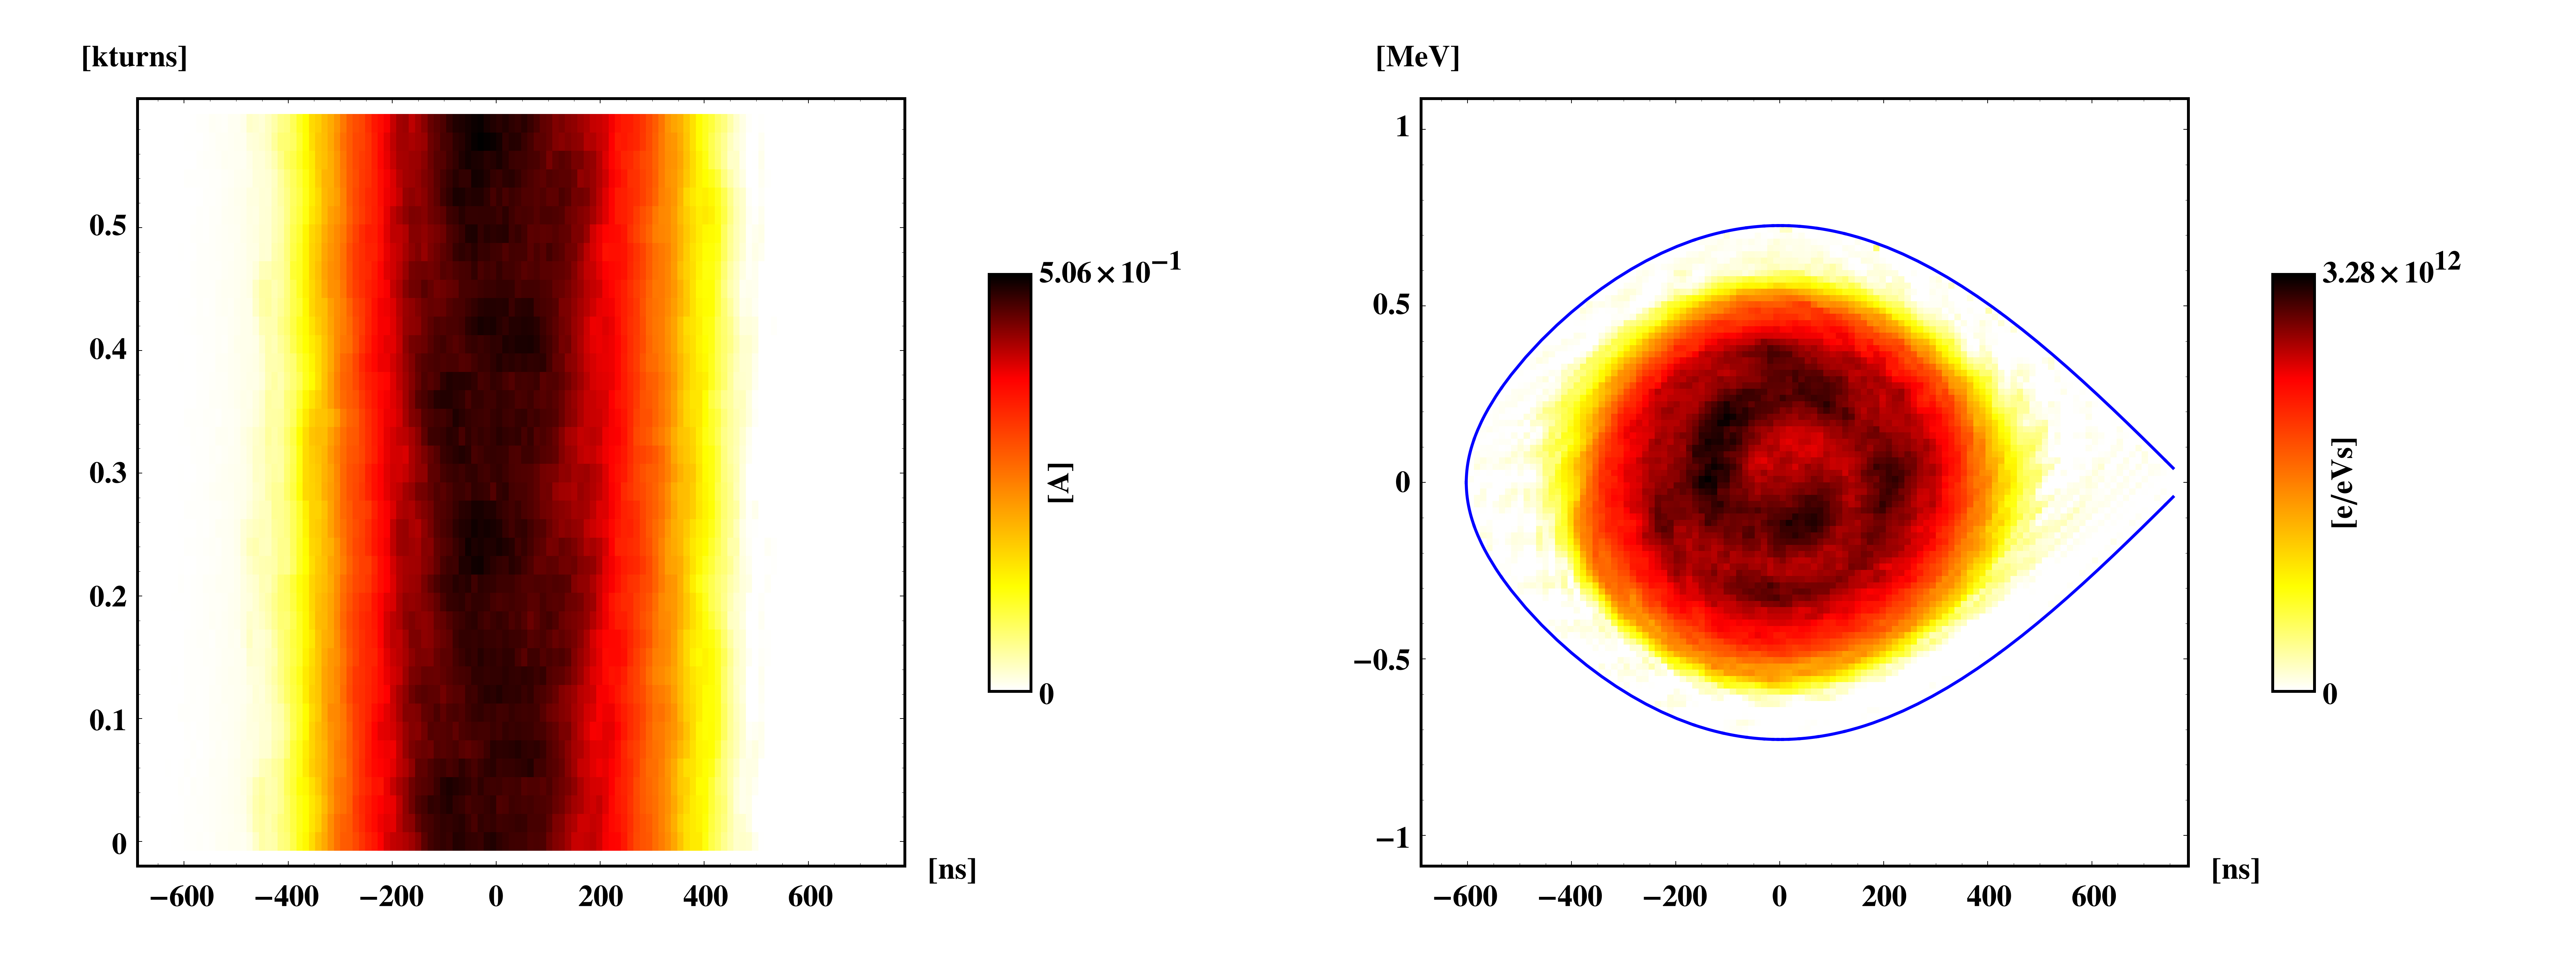
\includegraphics[width=\linewidth]{StateOfArt/Tosca2016fig.png} 

\caption[Phase space tomography]{\label{fig:PST} Early example (1999) of a set of 1D bunch profile data (left) processed into a 2D image of particle density in the longitudinal plane (right) using phase space tomography.  The resultant particle distribution is consistent with all the measured profiles and the physics of synchrotron motion.  The detailed internal bunch structure that is revealed is a consequence of the non-linearity of the motion.  The measurement was made at the CERN Proton Synchrotron Booster.\cite{pstweb}.} 
\end{center} 
\end{figure}


 Conceptually the method means adding the motion information to the geometry of the model with which the problem is posed rather than inserting it somehow into the mathematics of the tomography by which a solution is found. However, the specific technique used in phase space tomography is not viable in medical imaging, as the images are already very big in pixels, increasing the size e.g. 16 times would be computationally infeasible. Thus, the concept of phase space tomography must be implemented using a different method in CBCT.

\section{Motion in CBCT}
 Research into the removal of motion artefacts in CBCT is widespread and numerous articles have been published on the subject.  The most studied method to deal with motion is phase-correlated CBCT, also called 4D-CBCT\cite{sonke2005respiratory}\cite{thomas2006}\cite{li2006four}\cite{Pengpan2012246}\cite{t2016first}.  In 4D-CBCT, projection data are binned according to respiratory phase and then the data from each bin are reconstructed separately to produce a series of images.  This approach has several drawbacks.  Even though the amount of data per reconstructed image is smaller than usual, the total number of projections increases which means a longer irradiation time and a higher dose for the patient, limiting its clinical use.  In addition, the image quality of each 4D-CBCT reconstruction is inferior to a 3D-CBCT one due to its reduced angular sampling and to small inconsistencies resulting from binning inaccuracies. 

Due to the limitations of standard 4D-CBCT imaging, extensive research has been conducted to improve the quality of the images.  This work can be divided into two main groups: algorithmic approaches and deformation vector field (DVF) optimization methods.  Methods in the first group rely on regularization and other similar approaches.  An example is the work by Jia \textit{et al.}\cite{jia2012}, who implemented a non-local means of reconstruction to improve the temporal similarity between images.  Total variation methods (TV)\cite{ASD_POCS}, which minimize gradients within an image, have also been proposed with a temporal dimension included in the gradient\cite{0031-9155-57-6-1517}.  Another method based on TV minimization is the so-called PICCS algorithm\cite{chen2008prior}\cite{0031-9155-53-20-006}\cite{chen2012time} (it is actually a regularizer), which minimizes the TV and the difference between the reconstructed image and a prior image.  This prior image is generally a CBCT reconstructed with motion artefacts.  PICCS can reconstruct 4D-CBCT images from highly undersampled datasets.  More complex algorithms have also been proposed, such as ROOSTER\cite{:/content/aapm/journal/medphys/41/2/10.1118/1.4860215}, where a series of regularizations and minimizations are performed inside a region of interest to create clear 4D images in that area.

The methods of the second group generally (but not always) rely on a previous high-quality 4D-CT treatment planning scan as the basis from which to compute the DVFs.  As breathing motion is neither truly periodic nor reproducible in a given patient over time, the DVFs are corrected by matching real projections with simulated ones.  Finally, when the best DVF is computed, a synthetic image is generated by deforming the prior high-quality CT scan.  Examples include the work of Brock \textit{et al.}\cite{brock2010} and Ren \textit{et al.}\cite{Ren20121584}, who managed to reduce the number of projections required to about 60 using non-linear conjugate-gradient methods.  In order to improve robustness and reduce the dimensionality of the problem, DVF principal component analysis methods have also been proposed\cite{zhang2010correction}.  Li \textit{et al.}\cite{:/content/aapm/journal/medphys/37/6/10.1118/1.3426002}\cite{:/content/aapm/journal/medphys/38/5/10.1118/1.3582693} demonstrated that good accuracy can be achieved using only a single projection for the DVF optimization.

Hybrids between DVF-based and algorithmic approaches also exist, such as using TV regularization methods to improve convergence by initializing the DVFs\cite{wang2012high} or using temporal regularization with DVFs to improve the ROOSTER algorithm\cite{mory2016motion}.  Hybrid methods can lead to highly complex optimization strategies.  Examples include segmented mesh-based 4D-CBCT\cite{0031-9155-61-3-996} and the separation of static and moving images using TV, tight frame regularization and DVF optimization\cite{0031-9155-56-11-002}.  In addition, Christoffersen \textit{et al.}\cite{christoffersen2013registration} have proposed a multi-step algorithm using TV and optical flow for motion estimation.

Finally, some special mathematical algorithms have also been suggested that are unique in their approach.  These include the cine-CBCT algorithm\cite{6803058} and the 5D motion modelling approach\cite{0266-5611-31-11-115007}, which does not use phase-correlated binning.

The literature is full of these and many other approaches, ranging from the computationally and mathematically complex to those that sacrifice accuracy for simplicity and speed.  Most have been shown to yield good 4D-CBCT reconstructions, some in clinical scenarios.  But they all have drawbacks.  CBCT is a severely ill-posed problem where the amount of data is key for a good reconstruction.  The simplest methods that rely on binning will always suffer to some extent from a lack of data, even if temporal coherence is enforced with mathematical norms.  Additionally, they involve the reconstruction of several images, which is very expensive both computationally and in terms of memory.

Most DVF-based approaches ultimately use the DVFs to deform a prior image rather than using the acquired data directly to produce a reconstruction.  Further, they assume that a DVF can describe every possible anatomical change with respect to that prior image and this does not necessarily hold.

%{red}{\sout{Here, we propose a completely different approach to motion compensation in 4D-CT imaging.}}
In this work, a modelling method for motion compensation is presented, as first proposed by Hancock \textit{et al.}\cite{pst1} outside the medical domain and later independently proposed by Rit \textit{et al.}\cite{Rit1}\cite{Rit2} for CBCT. Since the publication of their work, computing on graphical processing units (GPUs) has taken a significant leap forward affording more modern techniques that can be used to reconstruct with greater accuracy and computational efficiency. With the use of GPUs even generic motion compensation is possible, without any numerical approximation of the weights in the projection and back projection and using better forward modelling\cite{fwdproj}. Such an approach is presented in this work.

This thesis focuses on thorax CBCT, but the method is generalizable to any X-ray absorption CT modality and to arbitrary motion.  The method requires no binning, but instead uses all projections to reconstruct an image at any respiratory phase.  It does require a sufficiently accurate description of the motion in terms of DVFs, but the approach is a modelling one so it can be used to introduce motion compensation into any iterative reconstruction algorithm. 

\section{Discussion}

Hopefully the topics presented in this chapter clarify why motion is a key problem to solve in IGRT and hadron therapy and why the solution should start by being able to image in 4D. The concepts in phase space tomography can not only  potentially solve the problem, but can do so by reducing the amount of data acquired significantly. This concept has barely been explored in the literature. Additionally, any general improvement on image quality in CBCT would not only benefit medical applications, but a entire set of different uses of the imaging technology.